\documentclass[a4paper]{article}

\usepackage[english]{babel}
\usepackage[utf8x]{inputenc}
\usepackage{amsmath}
\usepackage{amsfonts}
\usepackage{graphicx}
\usepackage{subfigure}
\usepackage{url}
\usepackage[colorinlistoftodos]{todonotes}

\title{CS 5785 -- Applied Machine Learning -- Lec.\ 4}
\author{Prof.\ Nathan Kallus, Cornell Tech\\Scribe: TBD}
\date{August 31, 2017}

\begin{document}
\maketitle

\section{The Newton-Raphson Method}
Logistic regression models are usually fit by maximum likelihood. As described at the end of last lecture, we will make use of its derivatives to maximize the log likelihood $\ell(\beta)$. This sets the stage for this optimization problem and brings us to a classic problem: root-finding, and a classic algorithm: Newton's method (also known as the Newton–Raphson method, named after Isaac Newton and Joseph Raphson). 

Fig.\ \ref{fig:newton} is an example of Newton's method from Wikipedia. To find the root of a function (shown in blue), we start with an initial guess $x_1$ and fit a tangent line using its first derivative if it exists. The tangent line is an approximation of the function at that point. Then we get new point $x_2$, which is assumed to be the root. Because the function is complex and we can see it is off the correct root. Then we use $x_2$ as the next guess. We repeat the process until a sufficiently accurate value is reached. Note that this is only guaranteed to provide us a local optimum.

Fig.\ \ref{fig:newton2} shows an instance of a Newton-type methods that uses both the first and second derivatives for a 1D function to find a local maximum of function $f(x)$. We start with a guess at $x_k$. Instead of fitting a tangent line to the function to generate the next guess, we fit a local quadratic approximation, i.e., a function that has the same 1st and 2nd derivatives as the target function. We can easily solve for the maximum of this new function and obtain the next guess for the maximum, $x_k+d_k$. We repeat this process until convergence.

In our case we wish to solve the related problem of finding the maximum of a function. We will do this using both the first and second derivatives. In higher dimensions, as with our log likelihood $\ell(\beta)$ where $\beta\in\mathbb{R}^{p+1}$, the counterparts to the 1st and 2nd derivatives are the gradient and the Hessian, respectively.
 

\begin{equation}
\ell(\beta) = \sum_{i=1}^N \left \{ y_i \beta ^\top x_i -  log(1+ e^{\beta ^\top x_i}) \right \}
\label{eqn:llgrad}
	\end{equation}
    
\begin{figure}
\centering
\subfigure[Start with a guess $x_1$, find the tangent line using the first derivative, extrapolate to get next guess $x_2$.]{
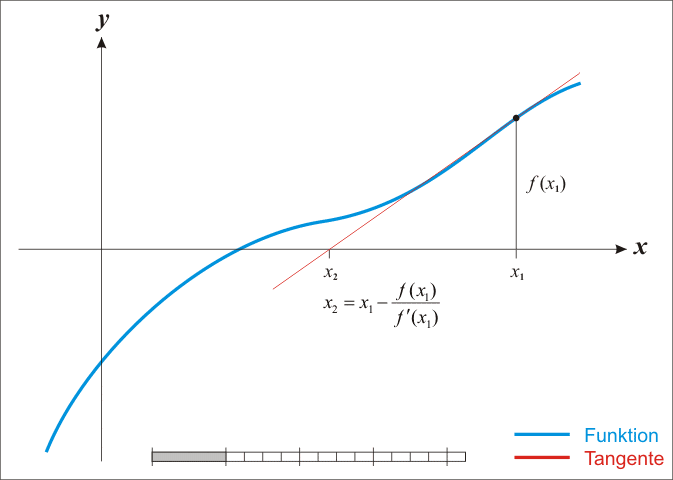
\includegraphics[width=0.45\textwidth]{NewtonIteration_Ani1.png}}
\quad
\subfigure[Repeat this process to get $x_3$, which as we can see overshoots in this case.]{
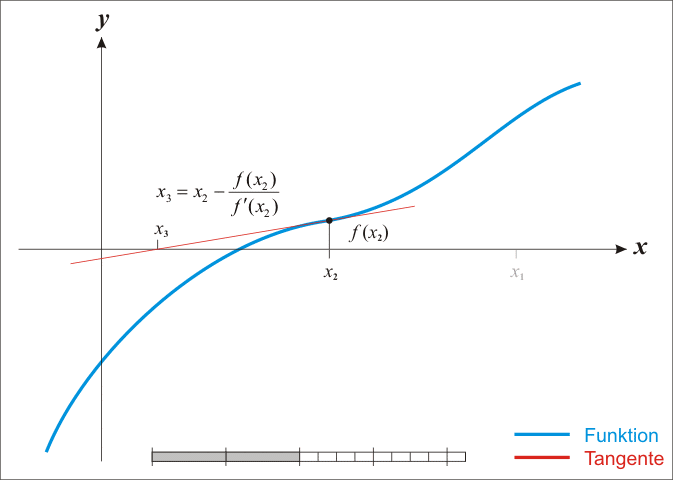
\includegraphics[width=0.45\textwidth]{NewtonIteration_Ani2.png}}

\subfigure[Keep iterating]{
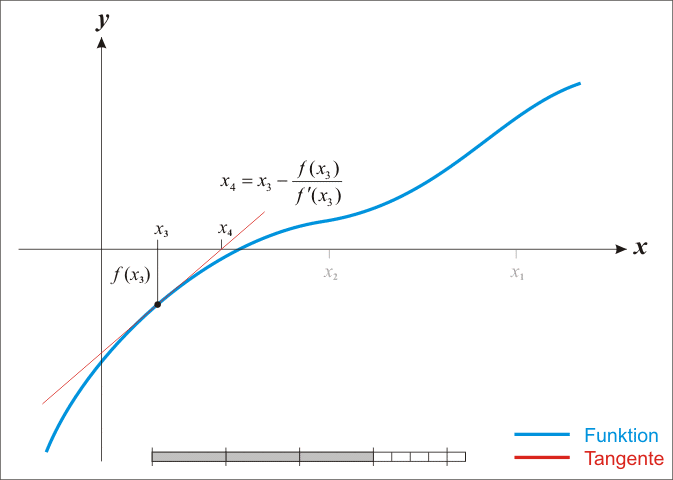
\includegraphics[width=0.45\textwidth]{NewtonIteration_Ani3.png}}
\quad
\subfigure[until a sufficiently accurate value is reached.]{
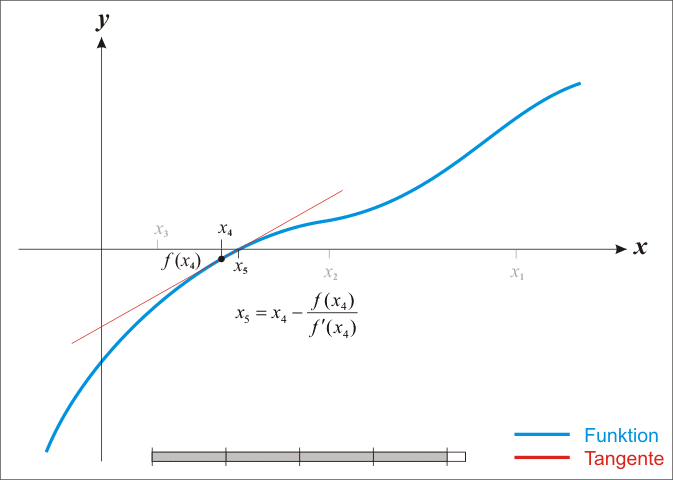
\includegraphics[width=0.45\textwidth]{NewtonIteration_Ani4.png}}
\caption{Illustration of Newton's method for finding a root. (Wikipedia)}
\label{fig:newton}
\end{figure}


\begin{figure}
\centering
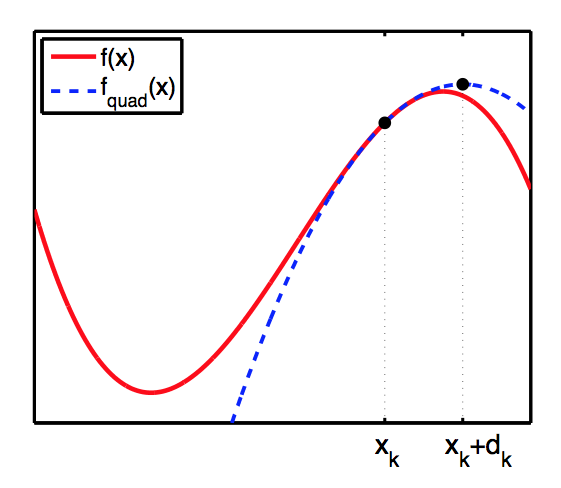
\includegraphics[width=0.6\textwidth]{newton_noncvx.png}
\caption{Finding a local maximum of a function $f(x)$ using a quadratic approximation.  We start with a guess at $x_k$.  Using both the 1st and 2nd order derivatives we fit a quadratic approximation to the function at that point.  That function $f_{\text{quad}}(x)$, is equivalent to the 2nd order Taylor series approximation of $f(x)$ around $x_k$.  We can easily solve for the maximum of this function and obtain the next guess for the maximum, $x_k+d_k$. We repeat this process until convergence. (Murphy)}
\label{fig:newton2}
\end{figure}


The gradient of the log likelihood is given by
\begin{equation}
\frac{\partial \ell(\beta)}{\partial \beta} = \sum_{i=1}^N x_i (y_i - p(x_i;\beta))
\label{eqn:llgrad}
	\end{equation}
Note that the gradient is a length $p+1$ vector.  We can see from this expression that the gradient can be expressed as a sum of feature vectors $x_i\in\mathbb{R}^{p+1}$, $i=1,\ldots,N$, weighted by $y_i-p(x_i;\beta)$.  We can interpret that weight as a signed error, since $p(x_i;\beta)$, the posterior probability, aims to approximate $y_i$.

The Hessian of $\ell(\beta)$, which is a $(p+1)\times(p+1)$ matrix, is given by
$$
\frac{\partial^2 \ell(\beta)}{\partial \beta\partial \beta^\top} = -\sum_{i=1}^N x_i x_i^\top p(x_i;\beta)\left(1-p(x_i;\beta)\right)
$$
This matrix is a sum of terms of the form $x_i x_i^\top$ weighted by $p(x_i;\beta)(1-p(x_i;\beta))$ and it characterizes the curvature of the function we're trying to minimize. Each $x_i x_i^\top$ term is the \textit{outer product} of $x_i$ with itself, resulting in a symmetric matrix of size $(p+1)\times(p+1)$.  We will see soon that this is closely related to how we compute the \emph{covariance matrix} for $\left\{x_i\right\}_1^N$. The scalar weight $p(x_i;\beta)(1-p(x_i;\beta))$ has a small value when $p(x_i;\beta)$ is close to $y_i$. If $p(x_i;\beta)$ is close to $1$ then $1 - p(x_i;\beta)$ is close to $0$ and vice versa, which means that if the approximation is good at least one multiplier in the expression $p(x_i;\beta)(1-p(x_i;\beta))$ is close to $0$. As a result, the entire expression has a very low value far from the decision boundary. If $p(x_i;\beta)$ is a bad approximation of $y_i$ there is a higher chance that the classification is incorrect and as such $p(x_i;\beta)$ is closer to $0.5$, $1 - p(x_i;\beta)$ is also close to $0.5$ making the entire expression close to its maximum: $0.25$. If we look back at the Hessian we can now see that the sum emphasizes $x_i$s for which we are less certain of their classification making the contribution to the Hessian  larger when the choice of $\beta$ results in a poor decision boundary. 

\begin{figure}
\centering
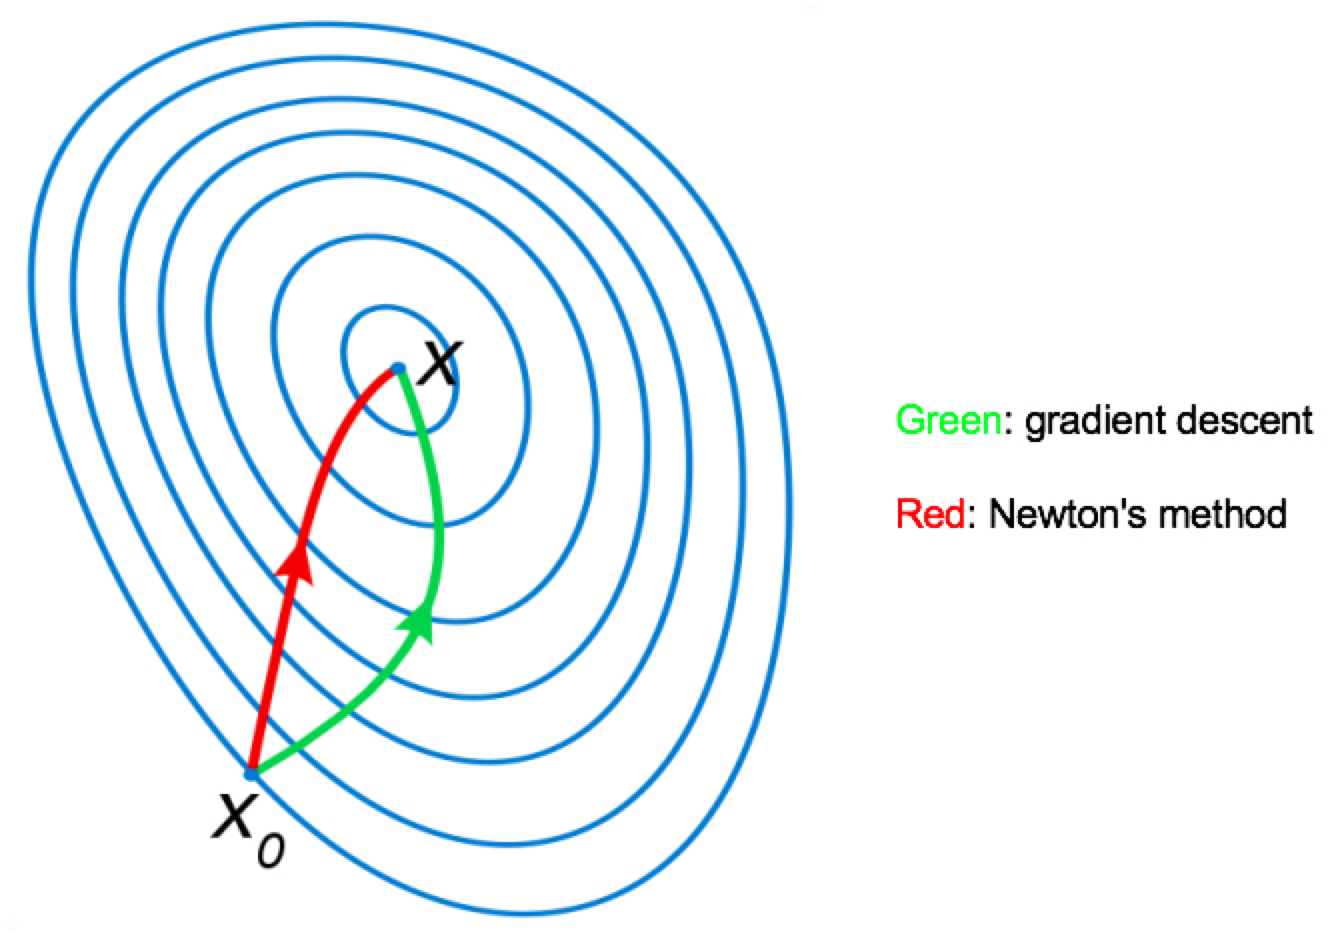
\includegraphics[width=1\textwidth]{Newton_s_Optimization.jpg}
\caption{A comparison of gradient descent (green) and Newton's method (red) for minimizing a function (with small step sizes). Newton's method uses curvature information to take a more direct route. (Wikipedia)}
\label{fig:newton3}
\end{figure}


Fig.\ \ref{fig:newton3} is a comparison of gradient descent (green) and Newton's method (red) for minimizing a function with small step sizes (the name of method varies depending on the reference) but the green curve is a classic first-order method and the red curve uses first- and second-order information. The first-order tells you something about the slope, and it will eventually get you to the local optimum by taking step in the direction of gradient. But if you take the curvature into account, which is indicated by the second-order derivative, you can get a more direct route. 


\subsection{Iterative Reweighted Least Squares (IRLS)}
In IRLS we start by picking a random choice for $\beta$ and apply a ``Newton update'' to get a better $\beta$. We continue taking Newton steps until we reach convergence. 
A Newton update is:
$$\beta^{new} = \beta^{old} - \left(\frac{\partial^2 \ell(\beta)}{\partial \beta\partial \beta^\top}\right)^{-1}\frac{\partial \ell(\beta)}{\partial \beta}$$
in which the derivatives are evaluated at $\beta=\beta^{old}$.  If we put this in matrix notation we get:
$$\frac{\partial \ell(\beta)}{\partial \beta} = \mathbf{X}^\top(\mathbf{y}-\mathbf{p})$$
$$\frac{\partial^2 \ell(\beta)}{\partial \beta\partial \beta^\top} = -\mathbf{X}^\top \mathbf{W}\mathbf{X}$$
Where:
\begin{itemize}
  \item $\mathbf{y}$ is a vector of all the $y_i$s.
  \item $\mathbf{X}\in\mathbb{R}^{N\times (p+1)}$ is the matrix of all the feature vectors $x_i$s.
  \item $\mathbf{p}$ is a vector of the $p(x_i;\beta)s$.
  \item $\mathbf{W}\in\mathbb{R}^{N\times N}$ is a diagonal weighting matrix containing the values of $p(x_i;\beta)(1-p(x_i;\beta))$ on the diagonal.
\end{itemize}
When we write the Newton update using this notation we get:
$$\beta^{new} = \beta+(\mathbf{X}^\top \mathbf{W}\mathbf{X})^{-1}\mathbf{X}^\top(\mathbf{y}-\mathbf{p})$$
$$\Downarrow$$
\begin{center}{(Multiply $\beta$ by $(\mathbf{X}^\top \mathbf{W}\mathbf{X})^{-1}(\mathbf{X}^\top \mathbf{W}\mathbf{X})$ which is the same as not changing it)}\end{center}
$$\beta^{new} = (\mathbf{X}^\top \mathbf{W}\mathbf{X})^{-1}(\mathbf{X}^\top \mathbf{W}\mathbf{X})\beta+(\mathbf{X}^\top \mathbf{W}\mathbf{X})^{-1}\mathbf{X}^\top(\mathbf{y}-\mathbf{p})$$
$$\Downarrow$$
\begin{center}(Factor out $(\mathbf{X}^\top \mathbf{W}\mathbf{X})^{-1}\mathbf{X}^\top \mathbf{W}$)\end{center}
$$\beta^{new} = (\mathbf{X}^\top \mathbf{W}\mathbf{X})^{-1}\mathbf{X}^\top \mathbf{W}(\mathbf{X}\beta+\mathbf{W}^{-1}(\mathbf{y}-\mathbf{p}))$$
$$\Downarrow$$
$$\beta^{new} = (\mathbf{X}^\top \mathbf{W}\mathbf{X})^{-1}\mathbf{X}^\top \mathbf{W}\mathbf{z}$$
in which $\mathbf{z}=\mathbf{X}\beta+\mathbf{W}^{-1}(\mathbf{y}-\mathbf{p})$. We call $\mathbf{z}$ the \textit{adjusted response}.\\
In every IRLS iteration we solve this equation with a new set of $\mathbf{p}$, $\mathbf{W}$ and $\mathbf{z}$. This iteration solves the following weighted least squares problem over and over:
$$\beta^{new}\leftarrow\underset{\beta}{\arg\min}(\mathbf{z}-\mathbf{X}\beta)^\top \mathbf{W}(\mathbf{z}-\mathbf{X}\beta)$$
(Recall $W$ is diagonal.)
We iterate this step until  convergence. 
This is named \emph{Iteratively Reweighted Least Squares} since in every iteration it solves a weighted least squares problem.

One remaining question is, how do we initialize $\beta$? Starting with $\beta=0$ is often OK.  Another option is to use multiple randomized restarts to reduce the chances of getting stuck at a local maximum.

\begin{itemize}
\item Pros: It's fast
\end{itemize}

\begin{itemize}
\item Cons: For each iteration need to invert a large matrix.
\item Cons: Need to include all observations in this matrix.
\end{itemize}

\begin{figure}
\centering
\subfigure{
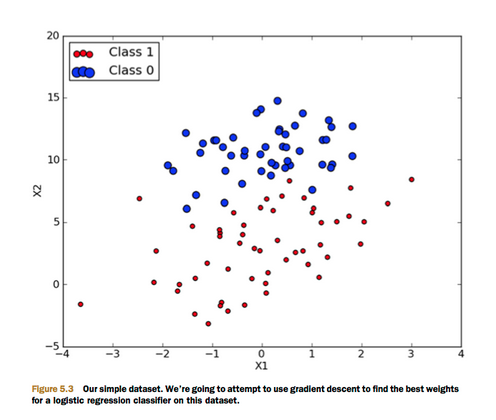
\includegraphics[width=0.45\textwidth]{HarringtonExample1.png}}
\quad
\subfigure{
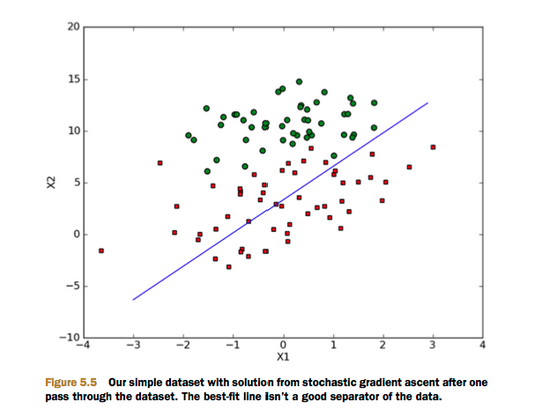
\includegraphics[width=0.45\textwidth]{HarringtonExample2.png}}

\subfigure{
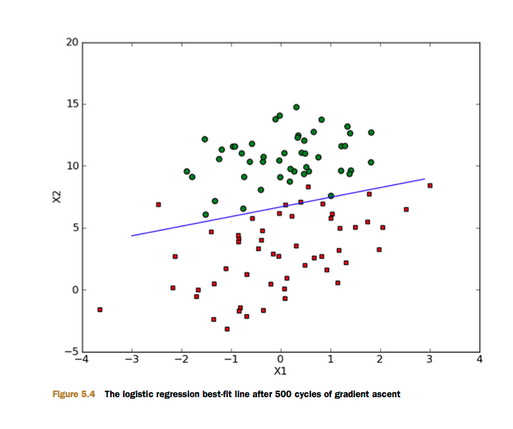
\includegraphics[width=0.45\textwidth]{HarringtonExample3.png}}
\quad
\caption{Logistic regression example (Harrington)}
\label{fig:Harrington}
\end{figure}


\section{Online Learning}
\subsection{Stochastic Gradient Descent}

IRLS is called a ``batch'' method since it has all the necessary data in advance, but that is not always possible or available.  For example, the data could be too big to fit into memory. Online learning updates $\beta$ every step based on individual streamed instances, as opposed to IRLS that uses all the data in every step. \emph{Stochastic Gradient Descent} (SGD) is an example of an online learning or streaming method that uses the following update step with \emph{step size} or \emph{learning rate} $\alpha$:
$$\beta^{new}\leftarrow \beta^{old}-\alpha x_i (y_i - p(x_i;\beta))$$
Compared to the exact expression for the gradient in Eqn.\ (\ref{eqn:llgrad}), SGD updates $\beta$ per data point rather than summing the gradient contributions over the entire data set.  If the data point was classified correctly the boundary doesn't change, if not we use the update rule above to update it.

Fig.\ \ref{fig:Harrington} is an example of SGD. We have two-class problem. The line presents the decision boundary. Every time it picks up a sample and checks that it is classified correctly or not. If correctly, the response is to do nothing. If incorrectly, it changes the boundary slightly to increase the likelihood. At the end, even the decision boundary is close to the example, it is considered as done.     

How do we choose the step size $\alpha$?  This is left as an exercise for the reader. 

\textbf{Perceptron Algorithm }
\todo[inline, color=green!40]{Technically that's perceptron learning; in this expression the update is proportional (including sign)  to the discrepancy between the ground truth and the estimated posterior probability.}
This algorithm is closely related to Rosenblatt's \emph{Perceptron Learning Algorithm} (HTF \S4.5.1), which is hard thresholded and doesn't maintain probability estimates.  See an example here: \url{http://www.youtube.com/watch?v=vGwemZhPlsA} (``Perceptron Learning Rule'').  The LMS algorithm of Widrow and Hoff is also an example of SGD. SGD are also used in training neural networks.


\begin{figure}
\centering
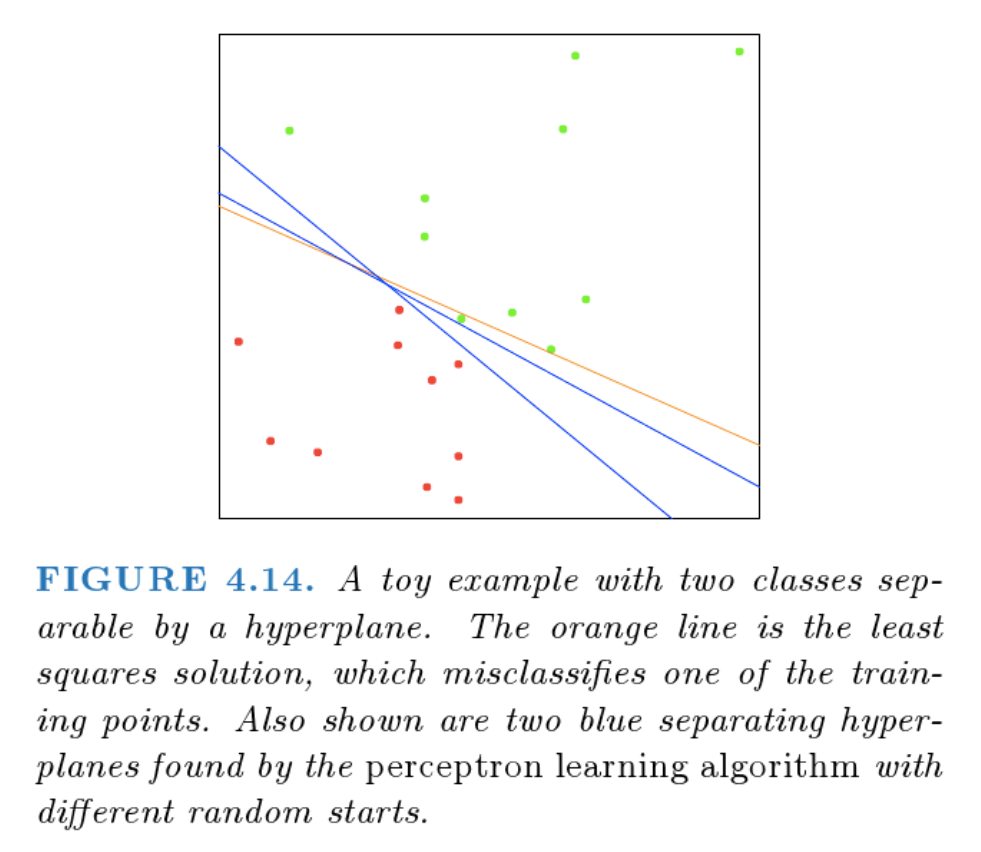
\includegraphics[width=0.75\textwidth]{sep_hyperplane}
\label{fig:sep_hyperplane}
\end{figure}

\subsection{Thoughts on Separating Hyperplanes}
As shown in HTF Fig.\ 4.14, given two classes that are linearly separable, there exists an infinite family of separating lines/planes/hyperplanes between the classes.  The figure shows solutions found via perceptron learning with different initializations.  Which solution is best?  Our intuition suggests we should choose the line with the furthest  perpendicular distance from the closest data points from each class, since this might prevent overfitting. How do we translate that into an algorithm?  We will tackle this question later in the semester when we discuss \emph{support vector machines}.

\subsection{Kernels: a Preview}
Note that so far we have just been using the input variables $X$ in their raw form (apart from adding the 1 to the front). A whole new frontier of algorithms awaits us if we supplement $x$ by squares and cross products of its variables like $x_1^2,x_2^2, x_1x_2$, etc. This hints at the idea of a \textit{kernel}, a mapping through which we can augment the representation by adding dimensionality. This is particularly useful when dealing with points that are not linearly separable, as in the XOR problem. We will discuss kernels later in the semester.


\section{Selected Q\&A}
\subsection{When do you use the first order approximation and when do you use the second order approximation?}
In practice, in very large big data machine learning contexts, people overwhelmingly use the first order approximation. Even though we know that the second order information is very very helpful and it infers the design of the algorithm, it has certain practical drawback that makes it harder to deploy. Every  iteration, you have to invert a large matrix and it is not really make things fast. 

\subsection{How do we know if we are stuck in local optimization and how to avoid it?}
You never know and could not solve it yet. It is a big problem in the filed. Now you can only have gigantic clusters doing random restarts and get the best local optima.  





\end{document}